\documentclass{standalone}
\usepackage[utf8]{inputenc}
\usepackage[T1]{fontenc}
\usepackage{graphicx}
\usepackage{color}
\usepackage{tikz}
\usepackage{pgfplots}
\pgfplotsset{compat=1.11}
\usetikzlibrary{patterns, pgfplots.fillbetween}

% f(x,y) = y
% c(x) = x*(x-1)*(x-2.3)*(x-3.3)+2.3

\begin{document}
  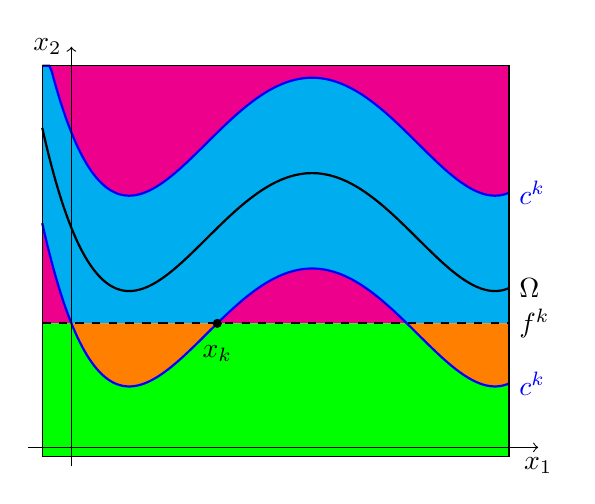
\begin{tikzpicture}
  \begin{axis}[axis lines=none,
      view={0}{90}, mark=none, samples=200, samples y=50,
      xmin=-0.3, xmax=3.4, ymin=-0.3, ymax=4.4,
      domain=-0.2:3]

    \addplot[name path=A, mark=none, draw=none]
        (x,4);
    \addplot[name path=B, mark=none, draw=none]
        (x,{min(4,0.5*x*(x-1)*(x-2.3)*(x-3.3)+3.3)});
    \addplot[name path=C, mark=none, draw=none]
        (x,{max(1.3,0.5*x*(x-1)*(x-2.3)*(x-3.3)+1.3});
    \addplot[name path=D, mark=none, draw=none]
        (x,1.3);
    \addplot[name path=E, mark=none, draw=none]
        (x,{min(1.3,0.5*x*(x-1)*(x-2.3)*(x-3.3)+1.3});
    \addplot[name path=F, mark=none, draw=none]
        (x,-0.1);

    \addplot[magenta] fill between[of=A and B];
    \addplot[cyan]    fill between[of=B and C];
    \addplot[magenta] fill between[of=C and D];
    \addplot[orange]  fill between[of=D and E];
    \addplot[green]   fill between[of=E and F];

    \addplot+[thick, mark=none, black]
        (x,{0.5*x*(x-1)*(x-2.3)*(x-3.3)+2.3})
        node[right] {$\Omega$};
    \addplot+[thick, mark=none, blue]
        (x,{min(4,0.5*x*(x-1)*(x-2.3)*(x-3.3)+3.3)})
        node[right] {$c^k$};
    \addplot+[thick, mark=none, blue]
        (x,{0.5*x*(x-1)*(x-2.3)*(x-3.3)+1.3})
        node[right] {$c^k$};
    \addplot+[thick, mark=none, black, dashed]
        (x,1.3) node[right] {$f^k$};
    \draw[->] (-0.3,0) -- (3.2,0) node[below] {$x_1$};
    \draw[->] (0,-0.2) -- (0,4.2) node[left] {$x_2$};
    \draw (-0.2,-0.1) rectangle (3,4);
    \draw[fill,circle] (1,1.3) node[below] {$x_k$} circle (0.05cm);
  \end{axis}
  \end{tikzpicture}
\end{document}
